\documentclass[11pt]{article}

% ============================================================
% Packages
% ============================================================

\usepackage[margin=1in]{geometry}

% Mathematics
\usepackage{amsmath}
\usepackage{amssymb}
\usepackage{mathtools}

% Figures and tables
\usepackage{graphicx}
\usepackage{booktabs}
\usepackage{float}
\usepackage{caption}
\usepackage{subcaption}

% Units and numbers
\usepackage{siunitx}

% Typography
\usepackage{microtype}

% Links and references
\usepackage{xcolor}
\usepackage[
colorlinks=true,
linkcolor=blue,
citecolor=blue,
urlcolor=blue
]{hyperref}

\usepackage[nameinlink,noabbrev]{cleveref}


% ============================================================
% Figure paths
% ============================================================

\graphicspath{
	{figures/}
	{figures/stage1/}
	{figures/stage2/}
	{figures/stage3/}
	{figures/stage4/}
	{figures/stage5/}
}


% ============================================================
% Document metadata
% ============================================================

\title{
	\textbf{Parallel Stochastic Filtering}\\[0.4em]
	\large From Shared-Memory Particle Filtering to Hybrid Parallel Methods
}

\author{
	Siddhartha Gupte\\
	Parallel Computing
}

\date{\today}


% ============================================================
% Document
% ============================================================

\begin{document}
	
	\maketitle
	
	\begin{abstract}
		
		This project studies stochastic filtering as a progressively more
		challenging parallel-computing problem. Beginning with a linear-Gaussian
		state-space model and an exact Kalman-filter benchmark, a bootstrap
		particle filter is developed, validated, and parallelized using OpenMP.
		Subsequent stages extend the framework to nonlinear filtering, parallel
		resampling, coupled fine--coarse simulations, distributed-memory
		execution with MPI, and hybrid MPI/OpenMP methods. The emphasis is on
		both numerical accuracy and computational scalability, with particular
		attention to synchronization, reductions, communication, and serial
		bottlenecks.
		
	\end{abstract}
	
	\tableofcontents
	\newpage
	
	
	% ============================================================
	% Report sections
	% ============================================================
	
	\section{Introduction}
\label{sec:introduction}

Stochastic filtering concerns the estimation of a time-varying hidden
state from noisy observations. The problem appears in many settings where
the quantity of interest cannot be measured directly but must instead be
inferred sequentially as new data arrive.

For linear systems with Gaussian noise, the filtering distribution can be
computed exactly using the Kalman filter. More general models typically
require numerical approximations. Particle filtering provides one such
approach by representing the filtering distribution with a collection of
weighted samples, or particles. Increasing the number of particles
improves the Monte Carlo approximation, but also increases the
computational cost.

Particle filters are particularly interesting from a parallel-computing
perspective. Propagation and likelihood evaluation can be carried out
independently across particles, while operations such as normalization,
estimation, and resampling require some form of global coordination.
The algorithm therefore contains both naturally parallel work and
potential scalability bottlenecks.

This project studies that interaction between filtering algorithms and
parallel computation. The work is organized in stages, with each stage
building on the previous implementation.

Stage~I uses a scalar linear-Gaussian model for which the Kalman filter
provides an exact benchmark. A bootstrap particle filter is first
validated against this reference solution and is then parallelized using
OpenMP. The resulting implementation is used to study race conditions,
reductions, strong scaling, and the effect of serial components on
end-to-end performance.

Later stages will extend the filtering and parallel-computing framework
as the project develops. The common questions are how accurately the
filter approximates the desired state distribution, which parts of the
algorithm can be parallelized effectively, and which operations ultimately
limit scalability.

Section~\ref{sec:background} summarizes the filtering concepts needed
for Stage~I. The remaining sections describe the individual stages,
their implementations, and their numerical and performance results.
	\section{Background}
\label{sec:background}

\subsection{State-Space Models and Bayesian Filtering}
\label{subsec:state-space-models}

A discrete-time state-space model consists of an unobserved state
\(X_t\) and an observation \(Y_t\),

\begin{align}
	X_t &\sim p(x_t\mid x_{t-1}), \\
	Y_t &\sim p(y_t\mid x_t).
\end{align}

The filtering problem is to compute the conditional distribution

\begin{equation}
	p(x_t\mid y_{0:t}),
\end{equation}

where \(y_{0:t}\) denotes all observations available through time \(t\).

The recursion consists of a prediction step,

\begin{equation}
	p(x_t\mid y_{0:t-1})
	=
	\int
	p(x_t\mid x_{t-1})
	p(x_{t-1}\mid y_{0:t-1})
	\,dx_{t-1},
\end{equation}

followed by a correction after observing \(y_t\),

\begin{equation}
	p(x_t\mid y_{0:t})
	\propto
	p(y_t\mid x_t)
	p(x_t\mid y_{0:t-1}).
\end{equation}


\subsection{Kalman Filtering}
\label{subsec:kalman-filter}

For a linear-Gaussian model,

\begin{align}
	X_t &= A X_{t-1} + \varepsilon_t,
	& \varepsilon_t &\sim \mathcal{N}(0,Q), \\
	Y_t &= C X_t + \eta_t,
	& \eta_t &\sim \mathcal{N}(0,R),
\end{align}

the filtering distribution remains Gaussian. It is therefore sufficient
to update its mean and variance.

If \(m_t^{-}\) and \(P_t^{-}\) denote the predictive mean and variance,
the scalar Kalman update is

\begin{align}
	K_t &=
	\frac{P_t^- C}{C^2P_t^-+R}, \\
	m_t &=
	m_t^- + K_t(Y_t-Cm_t^-), \\
	P_t &=
	(1-K_tC)P_t^-,
\end{align}

with prediction

\begin{align}
	m_{t+1}^- &= A m_t, \\
	P_{t+1}^- &= A^2P_t + Q.
\end{align}

For the linear-Gaussian model used in Stage~I, these recursions provide
the exact filtering mean and therefore a convenient benchmark.


\subsection{Particle Filtering}
\label{subsec:particle-filtering}

A particle filter approximates the filtering distribution using weighted
samples,

\begin{equation}
	p(x_t\mid y_{0:t})
	\approx
	\sum_{i=1}^{N}
	w_t^{(i)}
	\delta_{X_t^{(i)}}(x_t),
\end{equation}

with normalized weights satisfying

\begin{equation}
	\sum_{i=1}^{N} w_t^{(i)} = 1.
\end{equation}

In a bootstrap particle filter, particles are propagated using the state
transition,

\begin{equation}
	X_t^{(i)}
	\sim
	p(x_t\mid X_{t-1}^{(i)}),
\end{equation}

and weighted according to the observation likelihood,

\begin{equation}
	\widetilde{w}_t^{(i)}
	=
	p(y_t\mid X_t^{(i)}).
\end{equation}

After normalization,

\begin{equation}
	w_t^{(i)}
	=
	\frac{\widetilde{w}_t^{(i)}}
	{\sum_{j=1}^{N}\widetilde{w}_t^{(j)}},
\end{equation}

quantities such as the filtered mean can be estimated by

\begin{equation}
	\widehat{X}_t
	=
	\sum_{i=1}^{N} w_t^{(i)}X_t^{(i)}.
\end{equation}

The particle population is then resampled according to the normalized
weights. Since the method is Monte Carlo, its statistical error is
expected to decrease at the usual \(O(N^{-1/2})\) rate under standard
conditions.


\subsection{Parallel Structure}
\label{subsec:pf-parallel-structure}

Particle propagation and likelihood evaluation are independent across
particles and are therefore natural targets for data parallelism.
Normalization and posterior estimation require reductions over the
particle population, while resampling depends on the full set of
weights.

The distinction between particle-local work and global operations is the
main computational issue considered in Stage~I.
	
	% Stage I
	\newpage
	\section{Stage I: Linear-Gaussian Benchmark and Shared-Memory Particle Filtering}
\label{sec:stage1}

The first stage serves two purposes. First, it gives us a filtering
problem for which the correct answer is known: the linear-Gaussian model
can be solved exactly with a Kalman filter. Second, it gives us a simple
particle filter in which the sources of parallelism are easy to isolate.

The main question in this stage is therefore not only whether the particle
filter is numerically correct, but also which parts of the algorithm
benefit from shared-memory parallelism and which parts prevent the full
filter from scaling.


% ============================================================
\subsection{Stage-I Setup}
\label{subsec:stage1-setup}
% ============================================================

We use the scalar state-space model

\begin{align}
	X_t &= 0.9X_{t-1} + 0.5\varepsilon_t, \\
	Y_t &= X_t + \eta_t,
\end{align}

with

\begin{equation}
	\varepsilon_t,\eta_t\sim\mathcal{N}(0,1),
	\qquad
	X_0\sim\mathcal{N}(0,1).
\end{equation}

The simulation parameters are collected in
\cref{tab:stage1-parameters}.

\begin{table}[H]
	\centering
	\caption{Parameters used in the Stage-I state-space simulation.}
	\label{tab:stage1-parameters}
	\begin{tabular}{lc}
		\toprule
		Parameter & Value \\
		\midrule
		Number of time steps \(T\) & \(500\) \\
		State coefficient \(A\) & \(0.9\) \\
		Observation coefficient \(C\) & \(1.0\) \\
		State-noise standard deviation \(\sigma_x\) & \(0.5\) \\
		Observation-noise standard deviation \(\sigma_y\) & \(1.0\) \\
		Initial mean \(\mu_0\) & \(0.0\) \\
		Initial standard deviation \(\sigma_0\) & \(1.0\) \\
		\bottomrule
	\end{tabular}
\end{table}

A single trajectory of length \(T=500\) was generated and reused in all
experiments. The latent state is known because the data are simulated,
but neither filter receives it as input; both filters see only the
observations \(Y_t\).

For this model,

\begin{equation}
	Q=\sigma_x^2=0.25,
	\qquad
	R=\sigma_y^2=1,
\end{equation}

so the Kalman filter described in \cref{subsec:kalman-filter} gives the
exact filtering mean.

The bootstrap particle filter follows the usual cycle

\begin{equation}
	\text{propagate}
	\rightarrow
	\text{weight}
	\rightarrow
	\text{normalize}
	\rightarrow
	\text{estimate}
	\rightarrow
	\text{resample}.
\end{equation}

For the Gaussian observation model, the unnormalized particle weight is

\begin{equation}
	\widetilde{w}_t^{(i)}
	=
	\exp\left[
	-\frac{(Y_t-CX_t^{(i)})^2}{2\sigma_y^2}
	\right],
\end{equation}

and the filtered estimate is

\begin{equation}
	\widehat{X}_t^{\mathrm{PF}}
	=
	\sum_{i=1}^{N}
	w_t^{(i)}X_t^{(i)}.
\end{equation}

Multinomial resampling is used after each update. The state-space
simulation used seed \(42\), while the particle filter used a separate
seed \(12345\).


% ============================================================
\subsection{Numerical Validation}
\label{subsec:stage1-validation}
% ============================================================

Before parallelizing the particle filter, we first checked that it was
solving the filtering problem correctly.

Figure~\ref{fig:kalman-filter} shows the simulated state together with
the noisy observations and the Kalman estimate.

\begin{figure}[H]
	\centering
	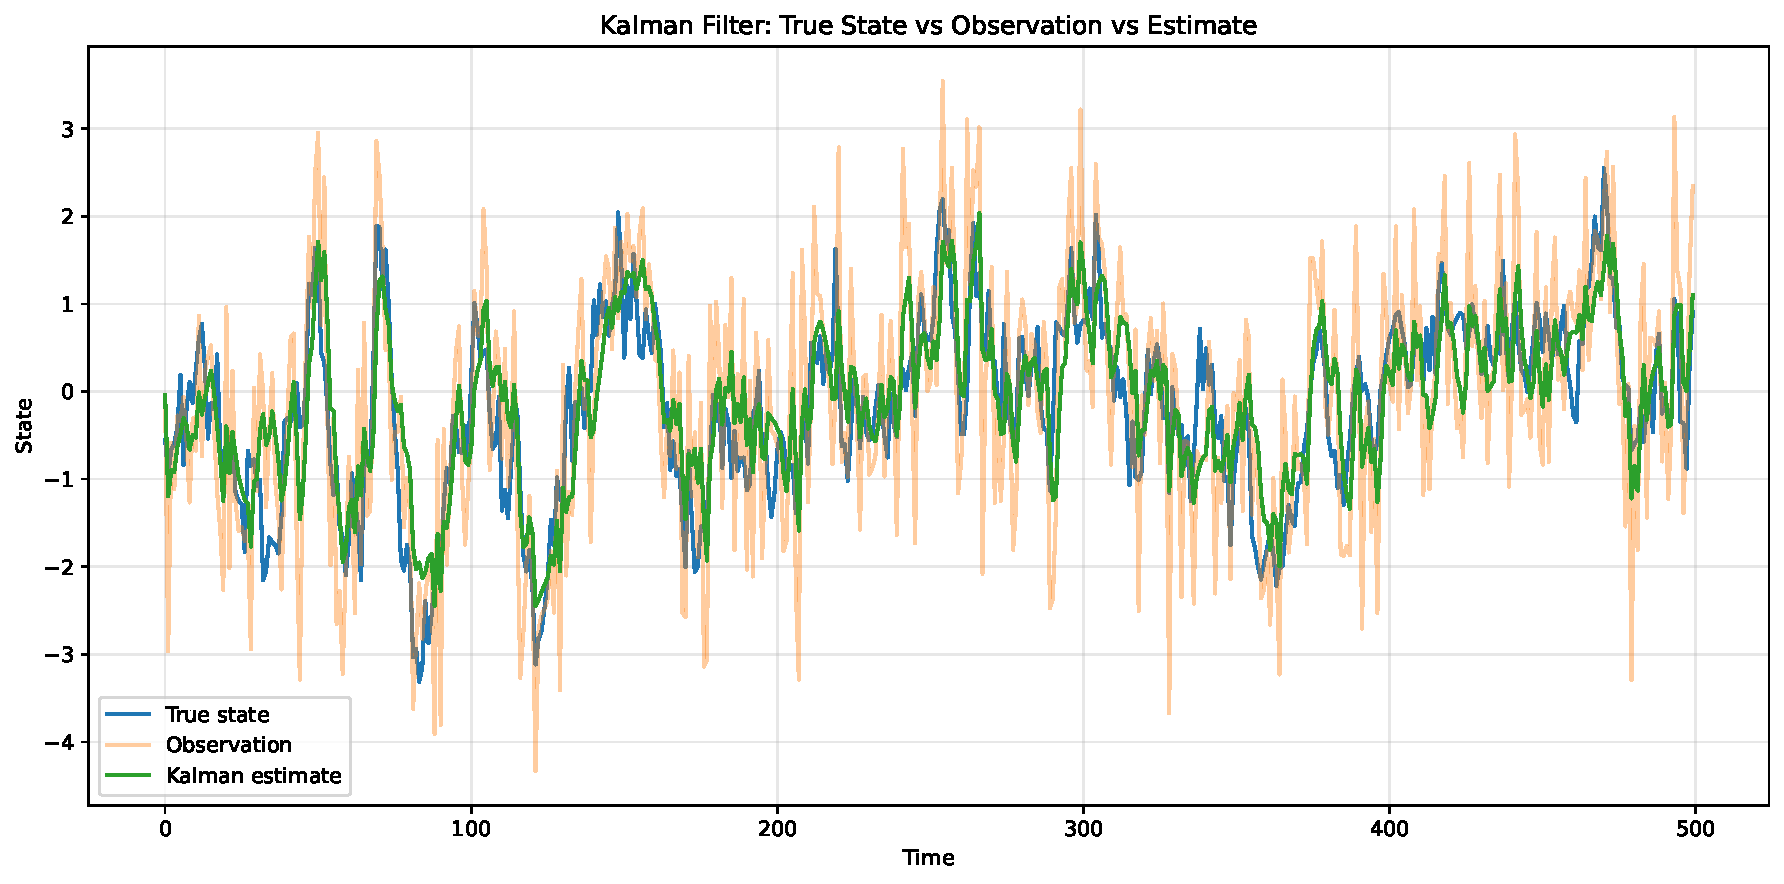
\includegraphics[width=0.92\textwidth]{kalman_filter.pdf}
	\caption{Simulated state, observations, and Kalman-filter estimate.}
	\label{fig:kalman-filter}
\end{figure}

The raw observations have an RMSE of \(1.029944\) relative to the true
state, while the Kalman estimate has an RMSE of \(0.616717\).

A particle filter with \(N=10{,}000\) particles gives nearly the same
trajectory as the Kalman filter, as shown in \cref{fig:filter-comparison}.

\begin{figure}[H]
	\centering
	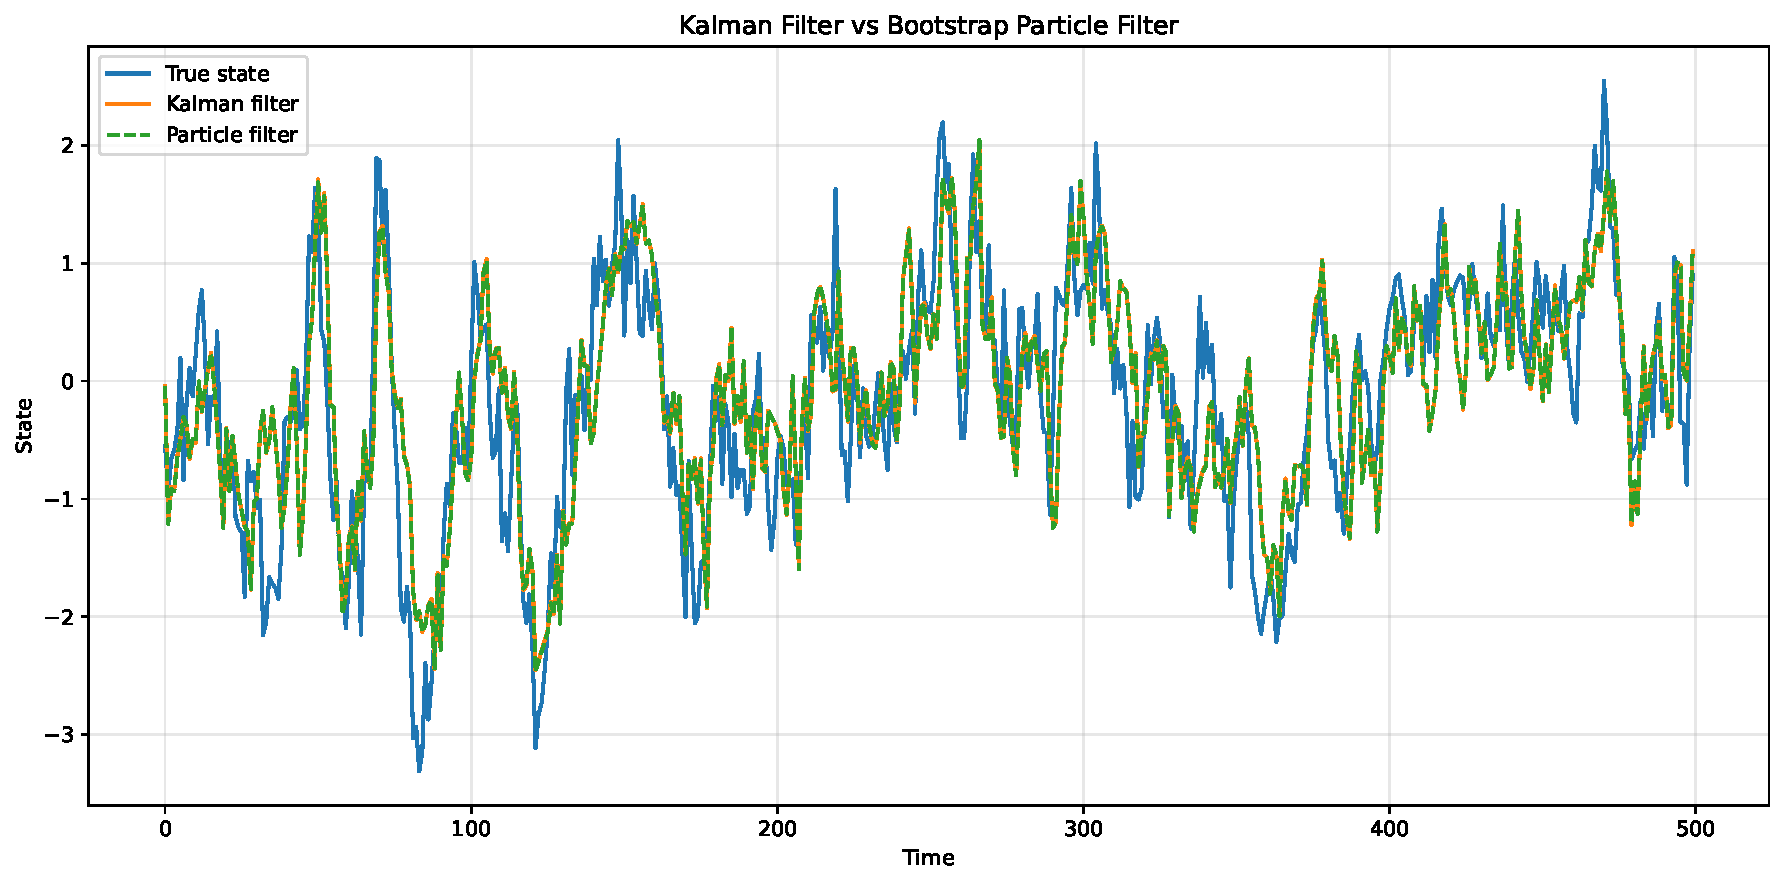
\includegraphics[width=0.92\textwidth]{filter_comparison.pdf}
	\caption{
		Kalman and bootstrap particle-filter estimates for
		\(N=10{,}000\).
	}
	\label{fig:filter-comparison}
\end{figure}

The main numerical checks are summarized in
\cref{tab:stage1-validation}.

\begin{table}[H]
	\centering
	\caption{Numerical validation of the serial particle filter.}
	\label{tab:stage1-validation}
	\begin{tabular}{lc}
		\toprule
		Quantity & RMSE \\
		\midrule
		Observations vs.\ true state & \(1.029944\) \\
		Kalman vs.\ true state & \(0.616717\) \\
		PF vs.\ true state, \(N=10{,}000\) & \(0.617360\) \\
		PF vs.\ Kalman, \(N=10{,}000\) & \(0.009906\) \\
		\bottomrule
	\end{tabular}
\end{table}

The more direct test of the particle approximation is the PF--Kalman
difference, since the Kalman mean is exact for this model. We therefore
repeated the serial particle filter over particle counts ranging from
\(100\) to \(500{,}000\).

\begin{figure}[H]
	\centering
	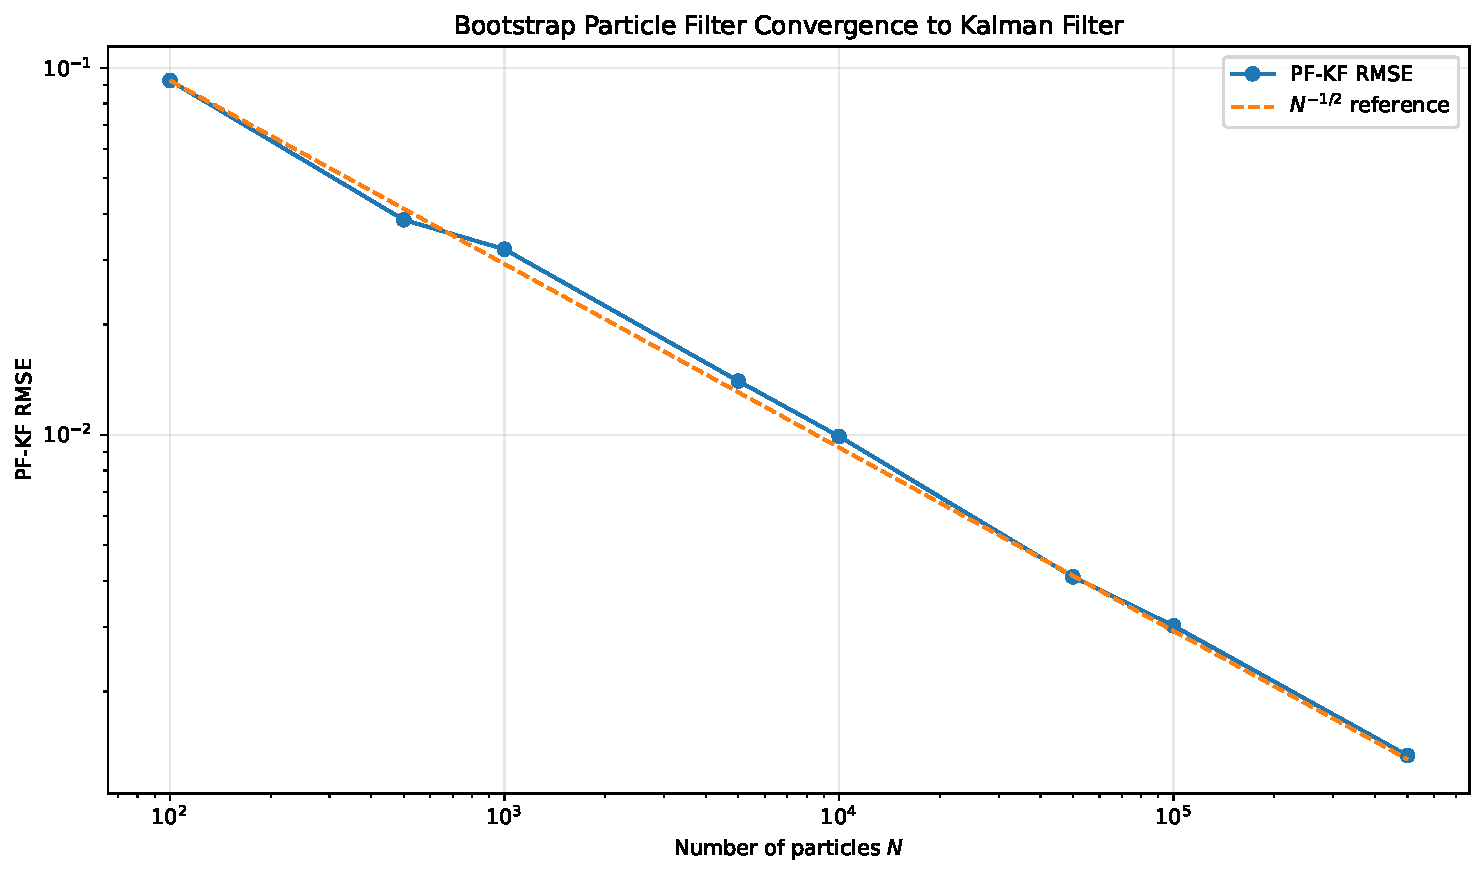
\includegraphics[width=0.82\textwidth]{serial_pf_convergence.pdf}
	\caption{
		PF--Kalman RMSE versus particle count. The dashed curve shows an
		\(N^{-1/2}\) reference rate.
	}
	\label{fig:pf-convergence}
\end{figure}

The log--log slope of the measured PF--Kalman RMSE is approximately

\begin{equation}
	-0.497,
\end{equation}

which is close to the expected Monte Carlo rate of \(-1/2\). This gives
us confidence that the serial implementation is behaving as expected
before introducing concurrency.


% ============================================================
\subsection{Parallelization Strategy}
\label{subsec:stage1-openmp}
% ============================================================

The particle index provides the natural source of data parallelism.
Once the particle population at time \(t-1\) is available, particle
\(i\) can be propagated independently,

\begin{equation}
	X_t^{(i)}
	=
	A X_{t-1}^{(i)}
	+
	\sigma_x\varepsilon_t^{(i)},
\end{equation}

and its likelihood can also be evaluated without reference to any other
particle. These loops were therefore parallelized with OpenMP using
static scheduling.

Not every step is particle-local, however. Weight normalization requires

\begin{equation}
	Z_t
	=
	\sum_{i=1}^{N}\widetilde{w}_t^{(i)},
\end{equation}

and the posterior mean requires

\begin{equation}
	\widehat{X}_t^{\mathrm{PF}}
	=
	\sum_{i=1}^{N}w_t^{(i)}X_t^{(i)}.
\end{equation}

Both are global reductions.

Random-number generation also needs some care. Sharing a single
\texttt{std::mt19937} engine between threads would itself require
synchronization. Instead, the implementation creates one generator per
OpenMP thread. Each thread accesses only its own engine while propagating
its assigned particles.

The Stage-I parallel structure is summarized in
\cref{tab:stage1-parallel-structure}.

\begin{table}[H]
	\centering
	\caption{Parallel structure of the Stage-I particle filter.}
	\label{tab:stage1-parallel-structure}
	\begin{tabular}{lc}
		\toprule
		Operation & Implementation \\
		\midrule
		Particle propagation & Parallel \\
		Likelihood evaluation & Parallel \\
		Weight summation & OpenMP reduction \\
		Weight normalization & Parallel \\
		Posterior mean & OpenMP reduction \\
		Multinomial resampling & Serial \\
		\bottomrule
	\end{tabular}
\end{table}

The last row is important. Resampling was deliberately left serial in
Stage~I. This lets us study the first layer of OpenMP parallelism without
also changing the resampling algorithm.


% ============================================================
\subsection{Synchronization and Reductions}
\label{subsec:stage1-synchronization}
% ============================================================

The weight sum provides a useful small experiment in parallel
correctness. Consider the apparently harmless loop

\begin{verbatim}
	#pragma omp parallel for
	for (...) {
		weight_sum += weights[i];
	}
\end{verbatim}

The addition is a read--modify--write operation on shared memory. Two
threads can read the same old value of \texttt{weight\_sum}, compute
different updates, and then overwrite one another. The result is a race
condition.

We tested three implementations of the same sum using
\(N=100{,}000\) particles and \(16\) threads.

For one fixed set of weights, the correct sum was

\begin{equation}
	70562.5.
\end{equation}

The naive implementation returned different values on repeated runs,
including \(8786.29\), \(13206.7\), and \(13243.8\).

A \texttt{critical} section fixes the race by allowing only one thread
at a time to update the accumulator. It is correct, but it also turns
the accumulation into a serial bottleneck. An OpenMP reduction avoids
this by giving each thread a private partial sum and combining those
partial sums at the end.

\begin{table}[H]
	\centering
	\caption{
		Weight-summation experiment for \(N=100{,}000\) and
		\(p=16\).
	}
	\label{tab:stage1-synchronization}
	\begin{tabular}{llll}
		\toprule
		Method & Correct? & Result & Observed cost \\
		\midrule
		Naive shared sum & No & Nondeterministic & -- \\
		\texttt{critical} & Yes & \(70562.5\) & \(8\)--\(12\) ms \\
		OpenMP reduction & Yes & \(70562.5\) & \(20\)--\(70\) \(\mu\)s \\
		\bottomrule
	\end{tabular}
\end{table}

This experiment is a useful example of the distinction between
\emph{thread safety} and \emph{parallel efficiency}. The critical
section makes the program correct, but correctness is achieved by
serializing every update. The reduction gives both correctness and a
parallel accumulation strategy.


% ============================================================
\subsection{Strong-Scaling Results}
\label{subsec:stage1-scaling}
% ============================================================

The strong-scaling tests were run on a 13th Gen Intel Core i7-13620H
with 10 physical cores and 16 logical CPUs. The code was compiled with
GCC~16.1.1 using C++23, OpenMP, and a Release build.

We tested

\begin{equation}
	N\in\{10^3,10^4,10^5,5\times10^5\}
\end{equation}

with

\begin{equation}
	p\in\{1,2,4,8,16\}
\end{equation}

OpenMP threads. Each configuration was run five times, and the median
wall-clock runtime was used.

Speedup and efficiency are defined by

\begin{equation}
	S_p=\frac{T_1}{T_p},
	\qquad
	E_p=\frac{S_p}{p}.
\end{equation}

\begin{figure}[H]
	\centering
	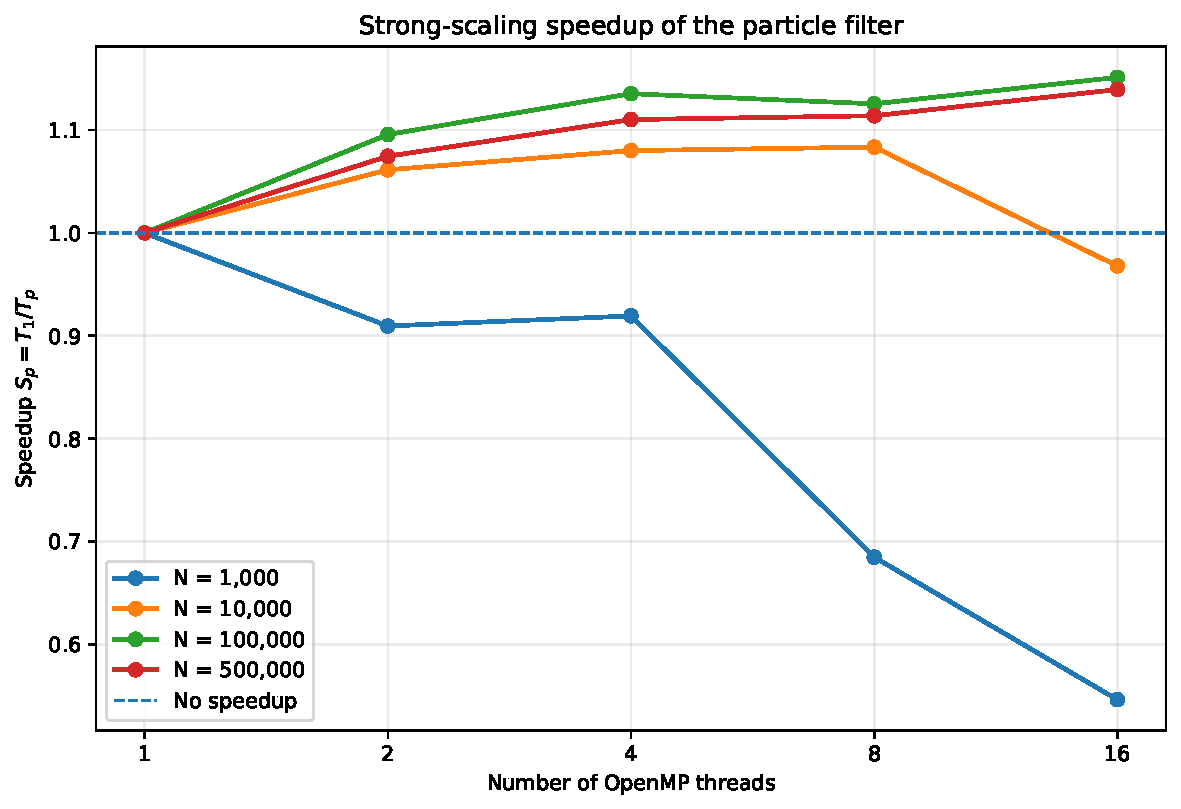
\includegraphics[width=0.86\textwidth]{openmp_speedup.pdf}
	\caption{
		Strong-scaling speedup for different particle counts.
		The dashed line marks the serial baseline \(S_p=1\).
	}
	\label{fig:openmp-speedup}
\end{figure}

The behavior depends strongly on problem size. At \(N=1{,}000\), the
OpenMP overhead is larger than the work saved by parallel execution, so
adding threads actually slows the filter down. By \(N=10{,}000\), a
small speedup appears. For the two largest populations, the improvement
is more consistent, although still modest.

A few representative values are shown in
\cref{tab:stage1-scaling-summary}.

\begin{table}[H]
	\centering
	\caption{Strong-scaling results at 16 OpenMP threads.}
	\label{tab:stage1-scaling-summary}
	\begin{tabular}{rrrr}
		\toprule
		\(N\) & Threads & Speedup & Efficiency \\
		\midrule
		\(1{,}000\)   & 16 & \(0.546\) & \(0.034\) \\
		\(10{,}000\)  & 16 & \(0.968\) & \(0.060\) \\
		\(100{,}000\) & 16 & \(1.151\) & \(0.072\) \\
		\(500{,}000\) & 16 & \(1.139\) & \(0.071\) \\
		\bottomrule
	\end{tabular}
\end{table}

The best end-to-end speedup is only about \(1.15\), despite using
16 threads.

\begin{figure}[H]
	\centering
	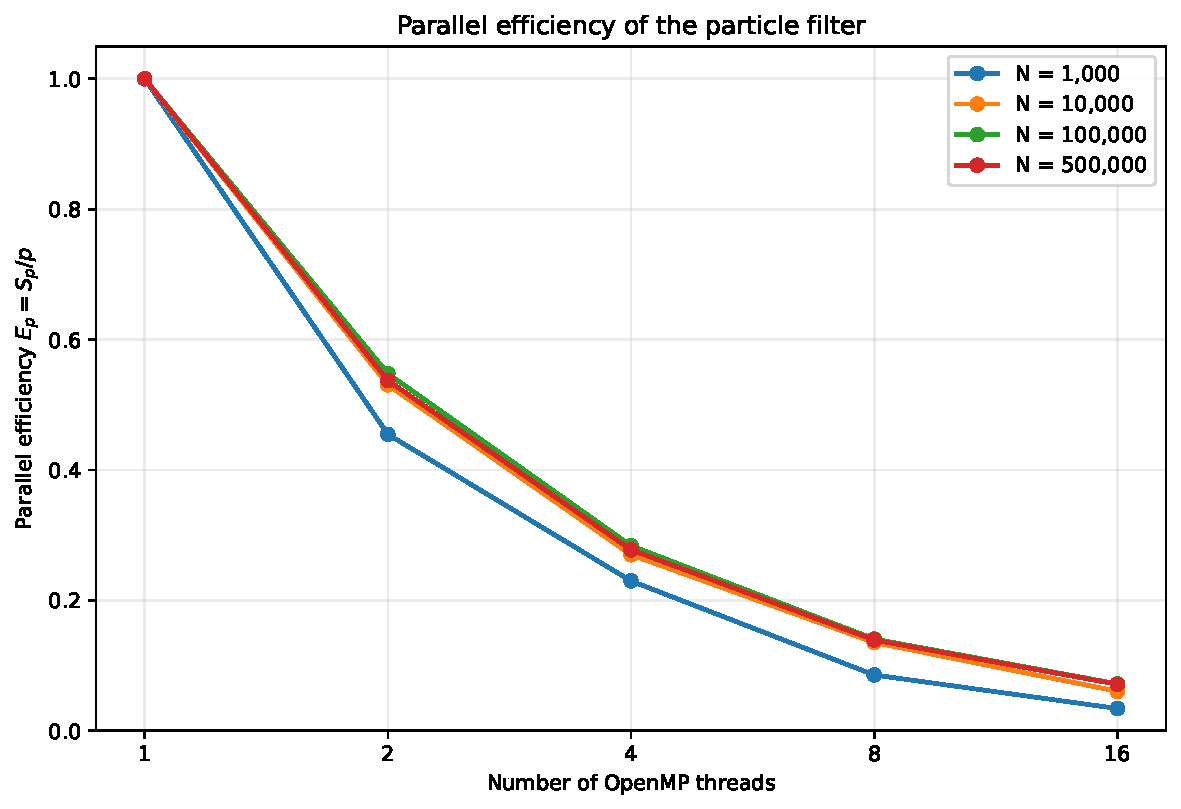
\includegraphics[width=0.86\textwidth]{openmp_efficiency.pdf}
	\caption{Parallel efficiency versus OpenMP thread count.}
	\label{fig:openmp-efficiency}
\end{figure}

The efficiency plot makes the same point from another angle. Even for
large particle populations, efficiency drops rapidly as threads are
added. This suggests that the limitation is not simply insufficient
particle-level work; some part of the full filter is not scaling with
the OpenMP kernels.


% ============================================================
\subsection{Where the Scaling Stops}
\label{subsec:stage1-runtime}
% ============================================================

To find the bottleneck, we timed the major pieces of the
\(N=500{,}000\) filter separately.

\begin{figure}[H]
	\centering
	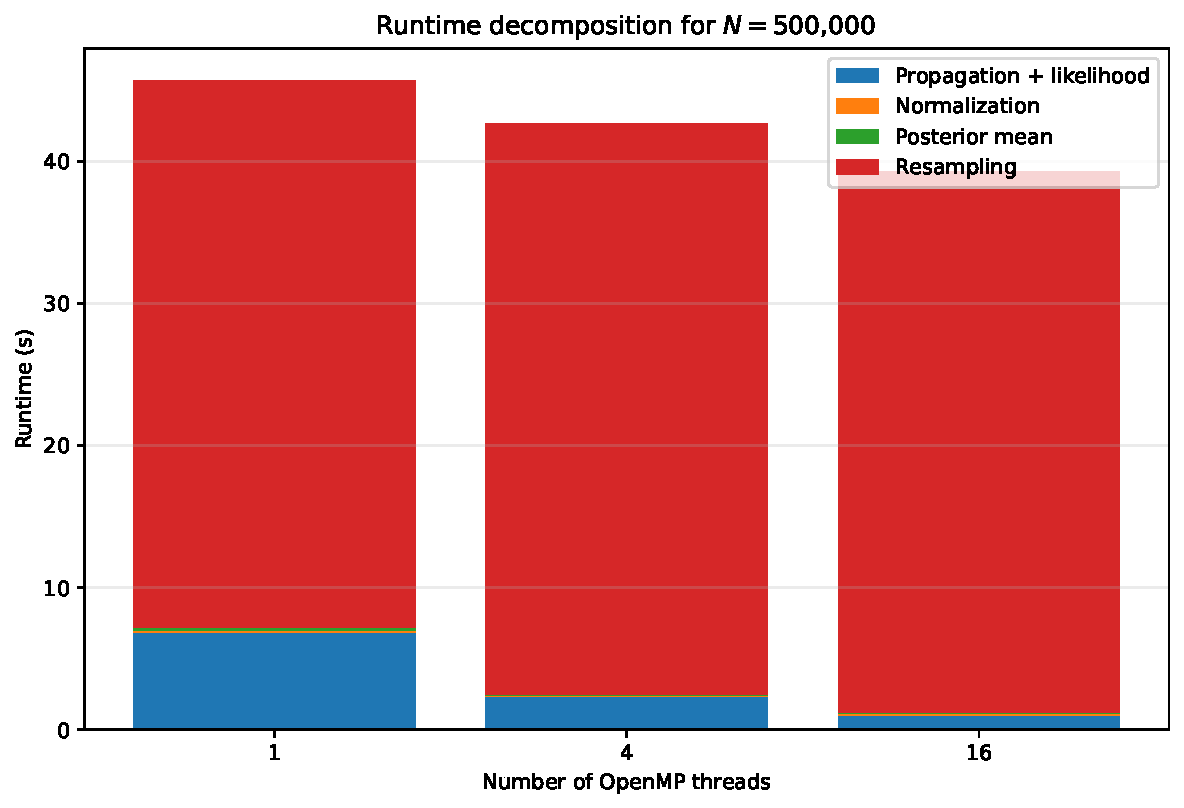
\includegraphics[width=0.86\textwidth]{openmp_runtime_breakdown.pdf}
	\caption{
		Runtime decomposition for \(N=500{,}000\).
	}
	\label{fig:openmp-runtime-breakdown}
\end{figure}

The raw measurements are given in
\cref{tab:stage1-runtime-breakdown}.

\begin{table}[H]
	\centering
	\caption{Runtime decomposition for \(N=500{,}000\), in seconds.}
	\label{tab:stage1-runtime-breakdown}
	\begin{tabular}{rrrrrr}
		\toprule
		Threads &
		Prop.+likelihood &
		Normalization &
		Posterior mean &
		Resampling &
		Total \\
		\midrule
		1  & 6.876 & 0.142 & 0.158 & 38.494 & 45.945 \\
		4  & 2.327 & 0.094 & 0.089 & 40.156 & 42.961 \\
		16 & 1.014 & 0.120 & 0.080 & 38.057 & 39.566 \\
		\bottomrule
	\end{tabular}
\end{table}

The interesting result is that the OpenMP kernel itself scales
reasonably well. Propagation and likelihood evaluation fall from
\(6.88\) s to \(1.01\) s between one and sixteen threads, a speedup of
about

\begin{equation}
	\frac{6.87557}{1.01447}\approx6.78.
\end{equation}

The full filter does not inherit that speedup because multinomial
resampling remains serial. Its runtime stays close to \(38\)--\(40\) s
regardless of the number of threads.

At one thread, resampling accounts for about \(84\%\) of the total
runtime. At sixteen threads, after the particle-local work has been
accelerated, that fraction rises to about \(96\%\).

This is precisely the situation described by Amdahl's law. If \(f\) is
the serial fraction,

\begin{equation}
	S_p
	\leq
	\frac{1}{f+(1-f)/p}.
\end{equation}

Taking \(f\approx0.84\) from the one-thread profile gives the rough
asymptotic limit

\begin{equation}
	S_\infty
	\approx
	\frac{1}{0.84}
	\approx1.19.
\end{equation}

The observed end-to-end speedup of about \(1.14\)--\(1.15\) is therefore
not surprising. The parallel kernel is getting faster; it is simply
becoming a smaller and smaller fraction of the total runtime.


% ============================================================
\subsection{Stage-I Summary}
\label{subsec:stage1-conclusions}
% ============================================================

Stage~I established a numerical and computational baseline for the rest
of the project.

The bootstrap particle filter converged toward the exact Kalman solution
at approximately the expected \(N^{-1/2}\) Monte Carlo rate.

The OpenMP implementation also exposed several basic shared-memory
issues directly. Particle-local work is straightforward to distribute,
random-number generators must be thread-local, and global sums require
proper reductions rather than unsynchronized shared updates. The
comparison between the naive sum, \texttt{critical}, and
\texttt{reduction} gave a concrete example of the difference between
correct synchronization and scalable synchronization.

Finally, the performance results showed why parallelizing only the
obvious loops is not enough. The propagation and likelihood kernel
achieved about \(6.8\times\) speedup at sixteen threads, while the
complete filter achieved only about \(1.15\times\). Serial resampling
was responsible for most of that gap.

The main outcome of Stage~I is therefore not simply an OpenMP particle
filter, but a clear picture of where its parallelism comes from and
where the current implementation stops scaling.
	
	% Stage II
	% \input{sections/section2}
	
	% Stage III
	% \input{sections/section3}
	
	% Stage IV
	% \input{sections/section4}
	
	% Stage V
	% \input{sections/section5}
	
	
	% ============================================================
	% Bibliography
	% ============================================================
	
	% We can add BibTeX/Biber once we begin citing literature.
	%
	% Example later:
	%
	% \bibliographystyle{plain}
	% \bibliography{references}
	
	
\end{document}